\documentclass[11pt, a4paper]{article}
\usepackage{pdfpages}
\usepackage{parallel}
\usepackage[T2A]{fontenc}
\usepackage{ucs}
\usepackage[utf8x]{inputenc}
\usepackage[polish,english,russian]{babel}
\usepackage{hyperref}
\usepackage{rotating}
\usepackage[inner=2cm,top=1.8cm,outer=2cm,bottom=2.3cm,nohead]{geometry}
\usepackage{listings}
\usepackage{graphicx}
\usepackage{wrapfig}
\usepackage{longtable}
\usepackage{indentfirst}
\usepackage{array}
\usepackage{tikzsymbols}
\usepackage{soul}
\usepackage[ruled,vlined]{algorithm2e}
%\counterwithout{figure}{section} 

\usepackage{url}
\makeatletter
\g@addto@macro{\UrlBreaks}{\UrlOrds}
\makeatother

\newcolumntype{P}[1]{>{\raggedright\arraybackslash}p{#1}}
\frenchspacing
\usepackage{fixltx2e} %text sub- and superscripts
\usepackage{icomma} % коскі ў матэматычным рэжыме
\PreloadUnicodePage{4}

\newcommand{\longpage}{\enlargethispage{\baselineskip}}
\newcommand{\shortpage}{\enlargethispage{-\baselineskip}}

\def\switchlang#1{\expandafter\csname switchlang#1\endcsname}
\def\switchlangbe{
\let\saverefname=\refname%
\def\refname{Літаратура}%
\def\figurename{Іл.}%
}
\def\switchlangen{
\let\saverefname=\refname%
\def\refname{References}%
\def\figurename{Fig.}%
}
\def\switchlangru{
\let\saverefname=\refname%
\let\savefigurename=\figurename%
\def\refname{Литература}%
\def\figurename{Рис.}%
}

\hyphenation{admi-ni-stra-tive}
\hyphenation{ex-pe-ri-ence}
\hyphenation{fle-xi-bi-li-ty}
\hyphenation{Py-thon}
\hyphenation{ma-the-ma-ti-cal}
\hyphenation{re-ported}
\hyphenation{imp-le-menta-tions}
\hyphenation{pro-vides}
\hyphenation{en-gi-neering}
\hyphenation{com-pa-ti-bi-li-ty}
\hyphenation{im-pos-sible}
\hyphenation{desk-top}
\hyphenation{elec-tro-nic}
\hyphenation{com-pa-ny}
\hyphenation{de-ve-lop-ment}
\hyphenation{de-ve-loping}
\hyphenation{de-ve-lop}
\hyphenation{da-ta-ba-se}
\hyphenation{plat-forms}
\hyphenation{or-ga-ni-za-tion}
\hyphenation{pro-gramming}
\hyphenation{in-stru-ments}
\hyphenation{Li-nux}
\hyphenation{sour-ce}
\hyphenation{en-vi-ron-ment}
\hyphenation{Te-le-pathy}
\hyphenation{Li-nux-ov-ka}
\hyphenation{Open-BSD}
\hyphenation{Free-BSD}
\hyphenation{men-ti-on-ed}
\hyphenation{app-li-ca-tion}

\def\progref!#1!{\texttt{#1}}
\renewcommand{\arraystretch}{2} %Іначай формулы ў матрыцы зліпаюцца з лініямі
\usepackage{array}

\def\interview #1 (#2), #3, #4, #5\par{

\section[#1, #3, #4]{#1 -- #3, #4}
\def\qname{LVEE}
\def\aname{#1}
\def\q ##1\par{{\noindent \bf \qname: ##1 }\par}
\def\a{{\noindent \bf \aname: } \def\qname{L}\def\aname{#2}}
}

\def\interview* #1 (#2), #3, #4, #5\par{

\section*{#1\\{\small\rm #3, #4. #5}}
\ifx\ParallelWhichBox\undefined%
    \addcontentsline{toc}{section}{#1, #3, #4}%
\else%
\ifnum\ParallelWhichBox=0%
    \addcontentsline{toc}{section}{#1, #3, #4}%
\fi\fi%

\def\qname{LVEE}
\def\aname{#1}
\def\q ##1\par{{\noindent \bf \qname: ##1 }\par}
\def\a{{\noindent \bf \aname: } \def\qname{L}\def\aname{#2}}
}

\newcommand{\interviewfooter}[1]{
\vskip 1em
\noindent \textit{#1}
}


\begin{document}

\title{1995 "--- Mouse Systems ProAgio / Genius EasyScroll Mouse}
\date{}
\maketitle

The Genius EasyScroll Mouse, also known as the Mouse Systems ProAgio Scroll Mouse, is the first mass-produced mouse with a scroll wheel. The mouse was released in 1995, five years after Mouse Systems was acquired by KYE, owner of the Genius brand.

\begin{figure}[h]
    \centering
    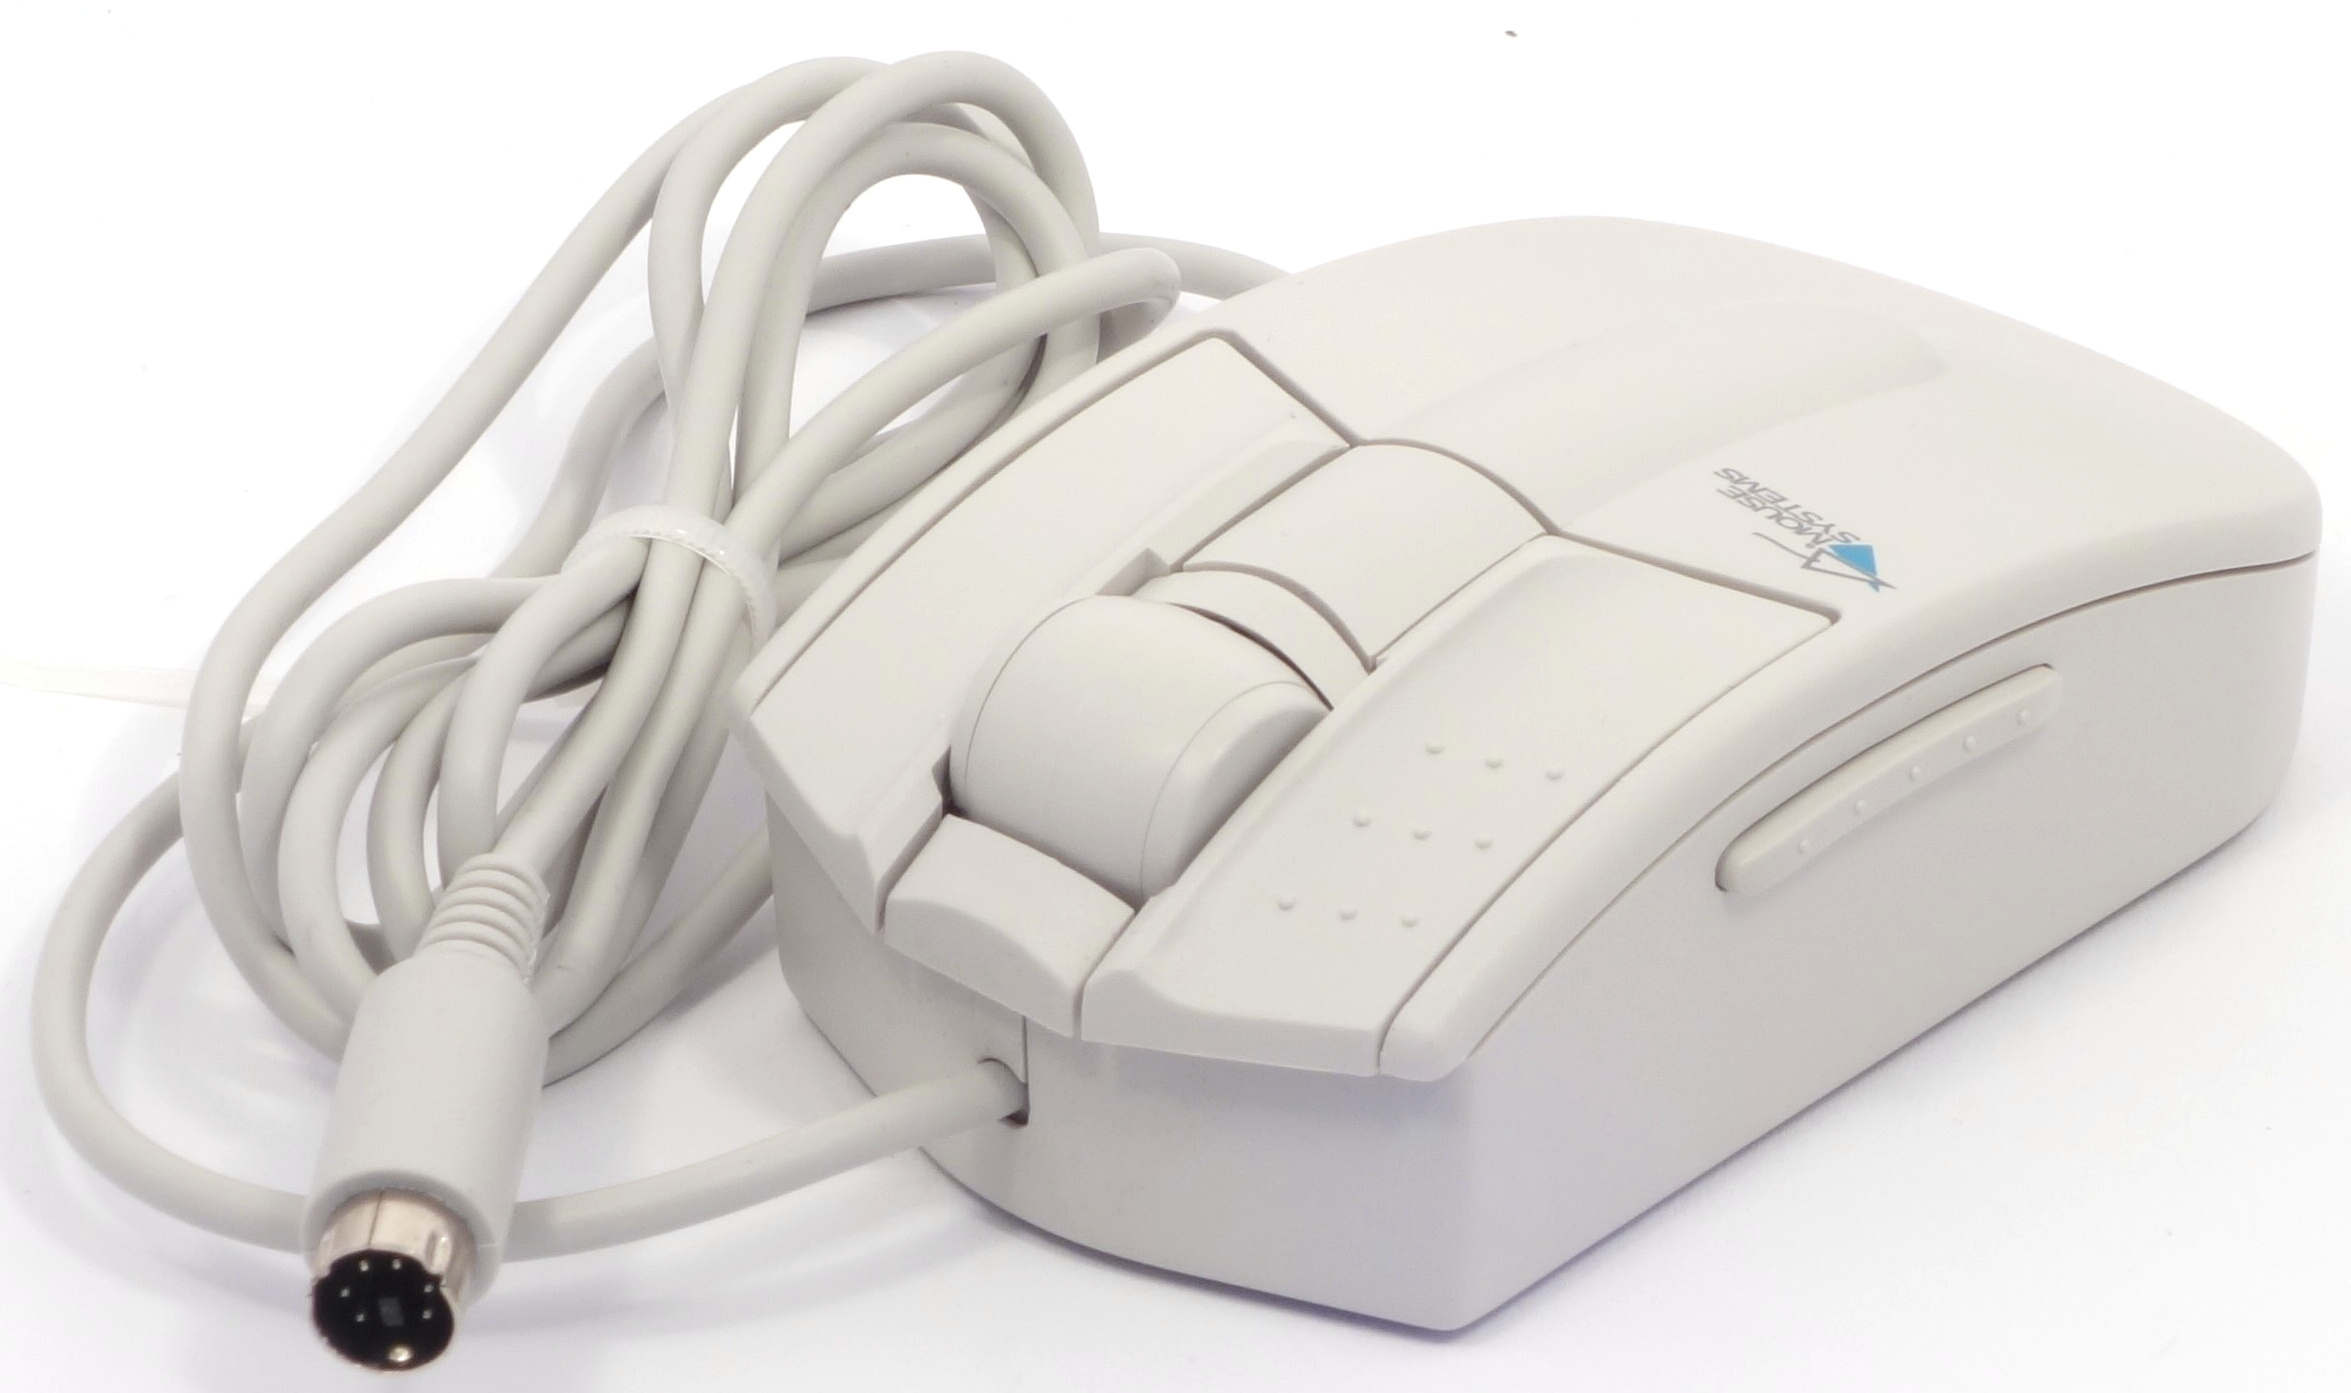
\includegraphics[scale=0.5]{1995_pro_agio_scroll_mouse/pic_30.jpg}
    \caption{ProAgio Scroll Mouse}
    \label{fig:ScrollPic}
\end{figure}


The mouse is ergonomically shaped (figure \ref{fig:ScrollPic}). The device has five fairly large buttons with ribbed edges, and the left button has an embossed surface for easier tactile identification. The scroll wheel is located in the middle of the case, farthest from the user, and is much wider than in later versions (in fact, it could not be called a wheel, but a roller or drum). In addition to the scrolling function, it reacts to pressing like a button, as in most later mice. In addition, a long narrow button on the side of the case is accessible to the user's thumb. \ref{fig:ScrollHand}. Presumably, button functions can be remapped using software \cite{yt}.

\begin{figure}[h]
    \centering
    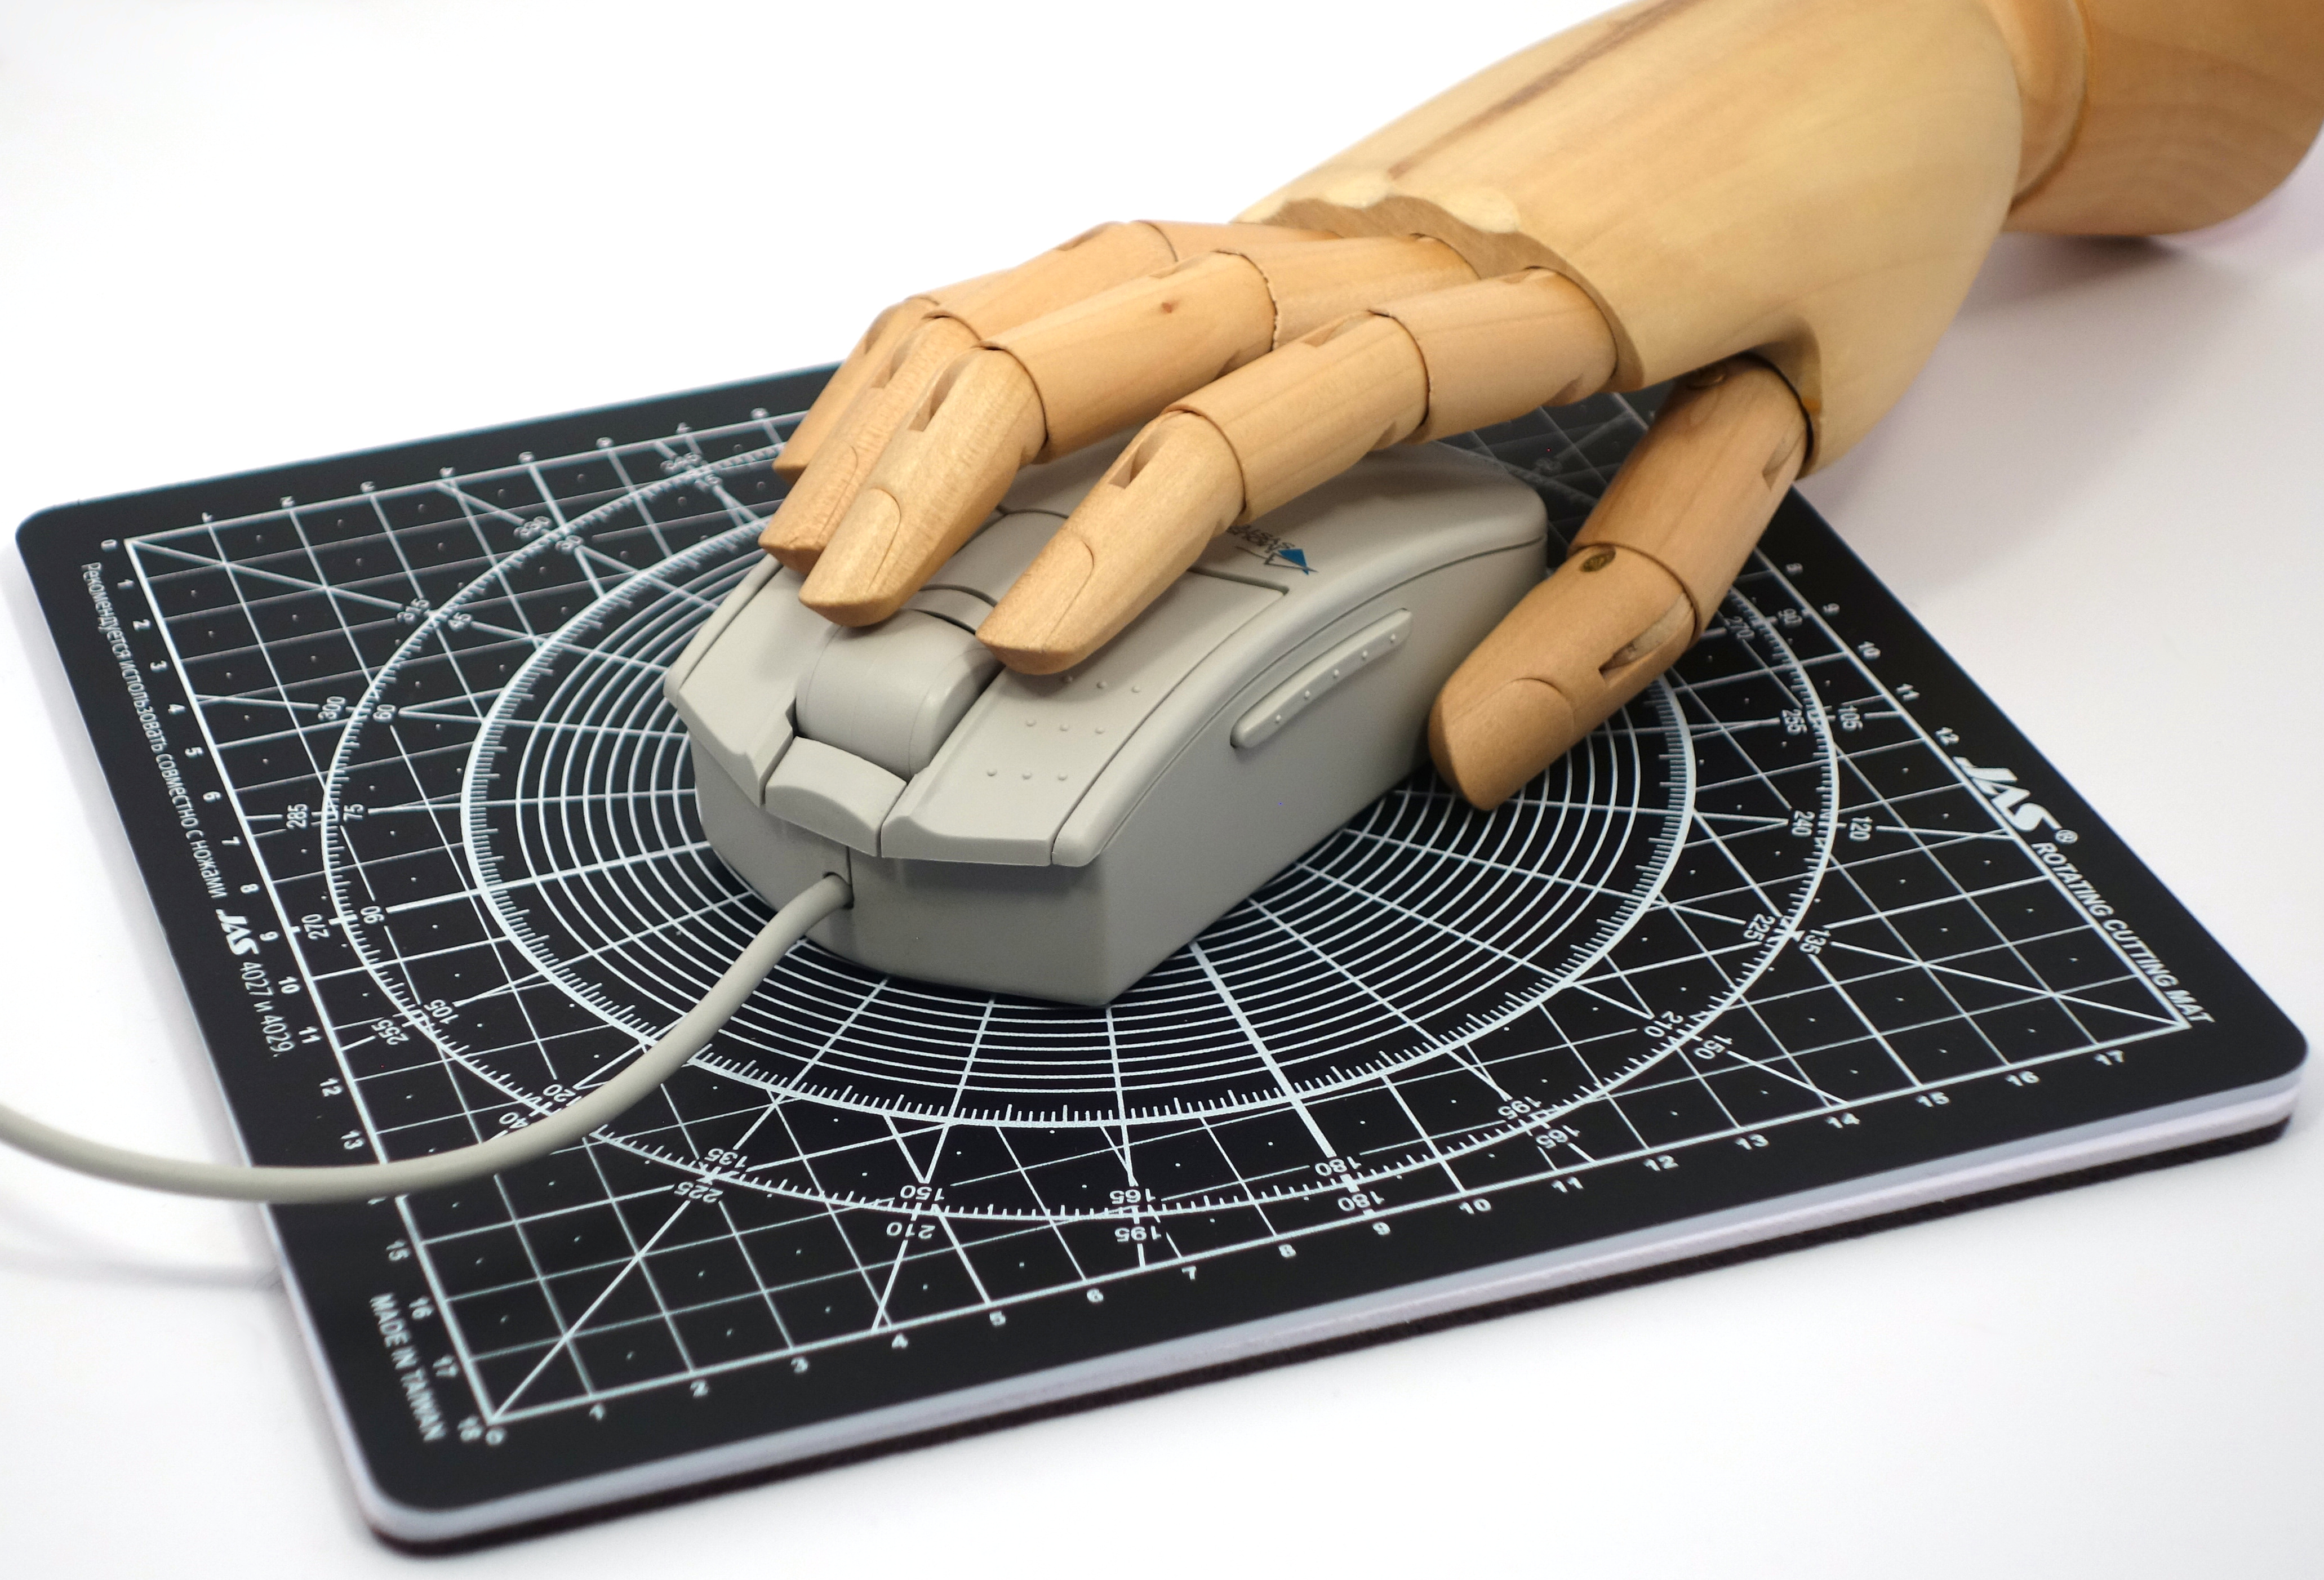
\includegraphics[scale=0.3]{1995_pro_agio_scroll_mouse/hand_30.jpg}
    \caption{ProAgio Scroll Mouse with a human hand model}
    \label{fig:ScrollHand}
    \end{figure}

It's worth noting that the idea of a finger-roller on a pointing device predates the ProAgio Scroll Mouse, but it's never been used to scroll text before. For example, the developers of the MicroSpeed FastTRAP trackball in 1987 used a wheel to control the \textit{z}-axis movement in 3D graphics software (the trackball ball traditionally provided movement along the \textit{x} and \textit{y} axes). In the FastTRAP white paper released by MicroSpeed, the wheel was described as “Trackwheel to indicate the third axis”.

\begin{figure}[h]
    \centering
    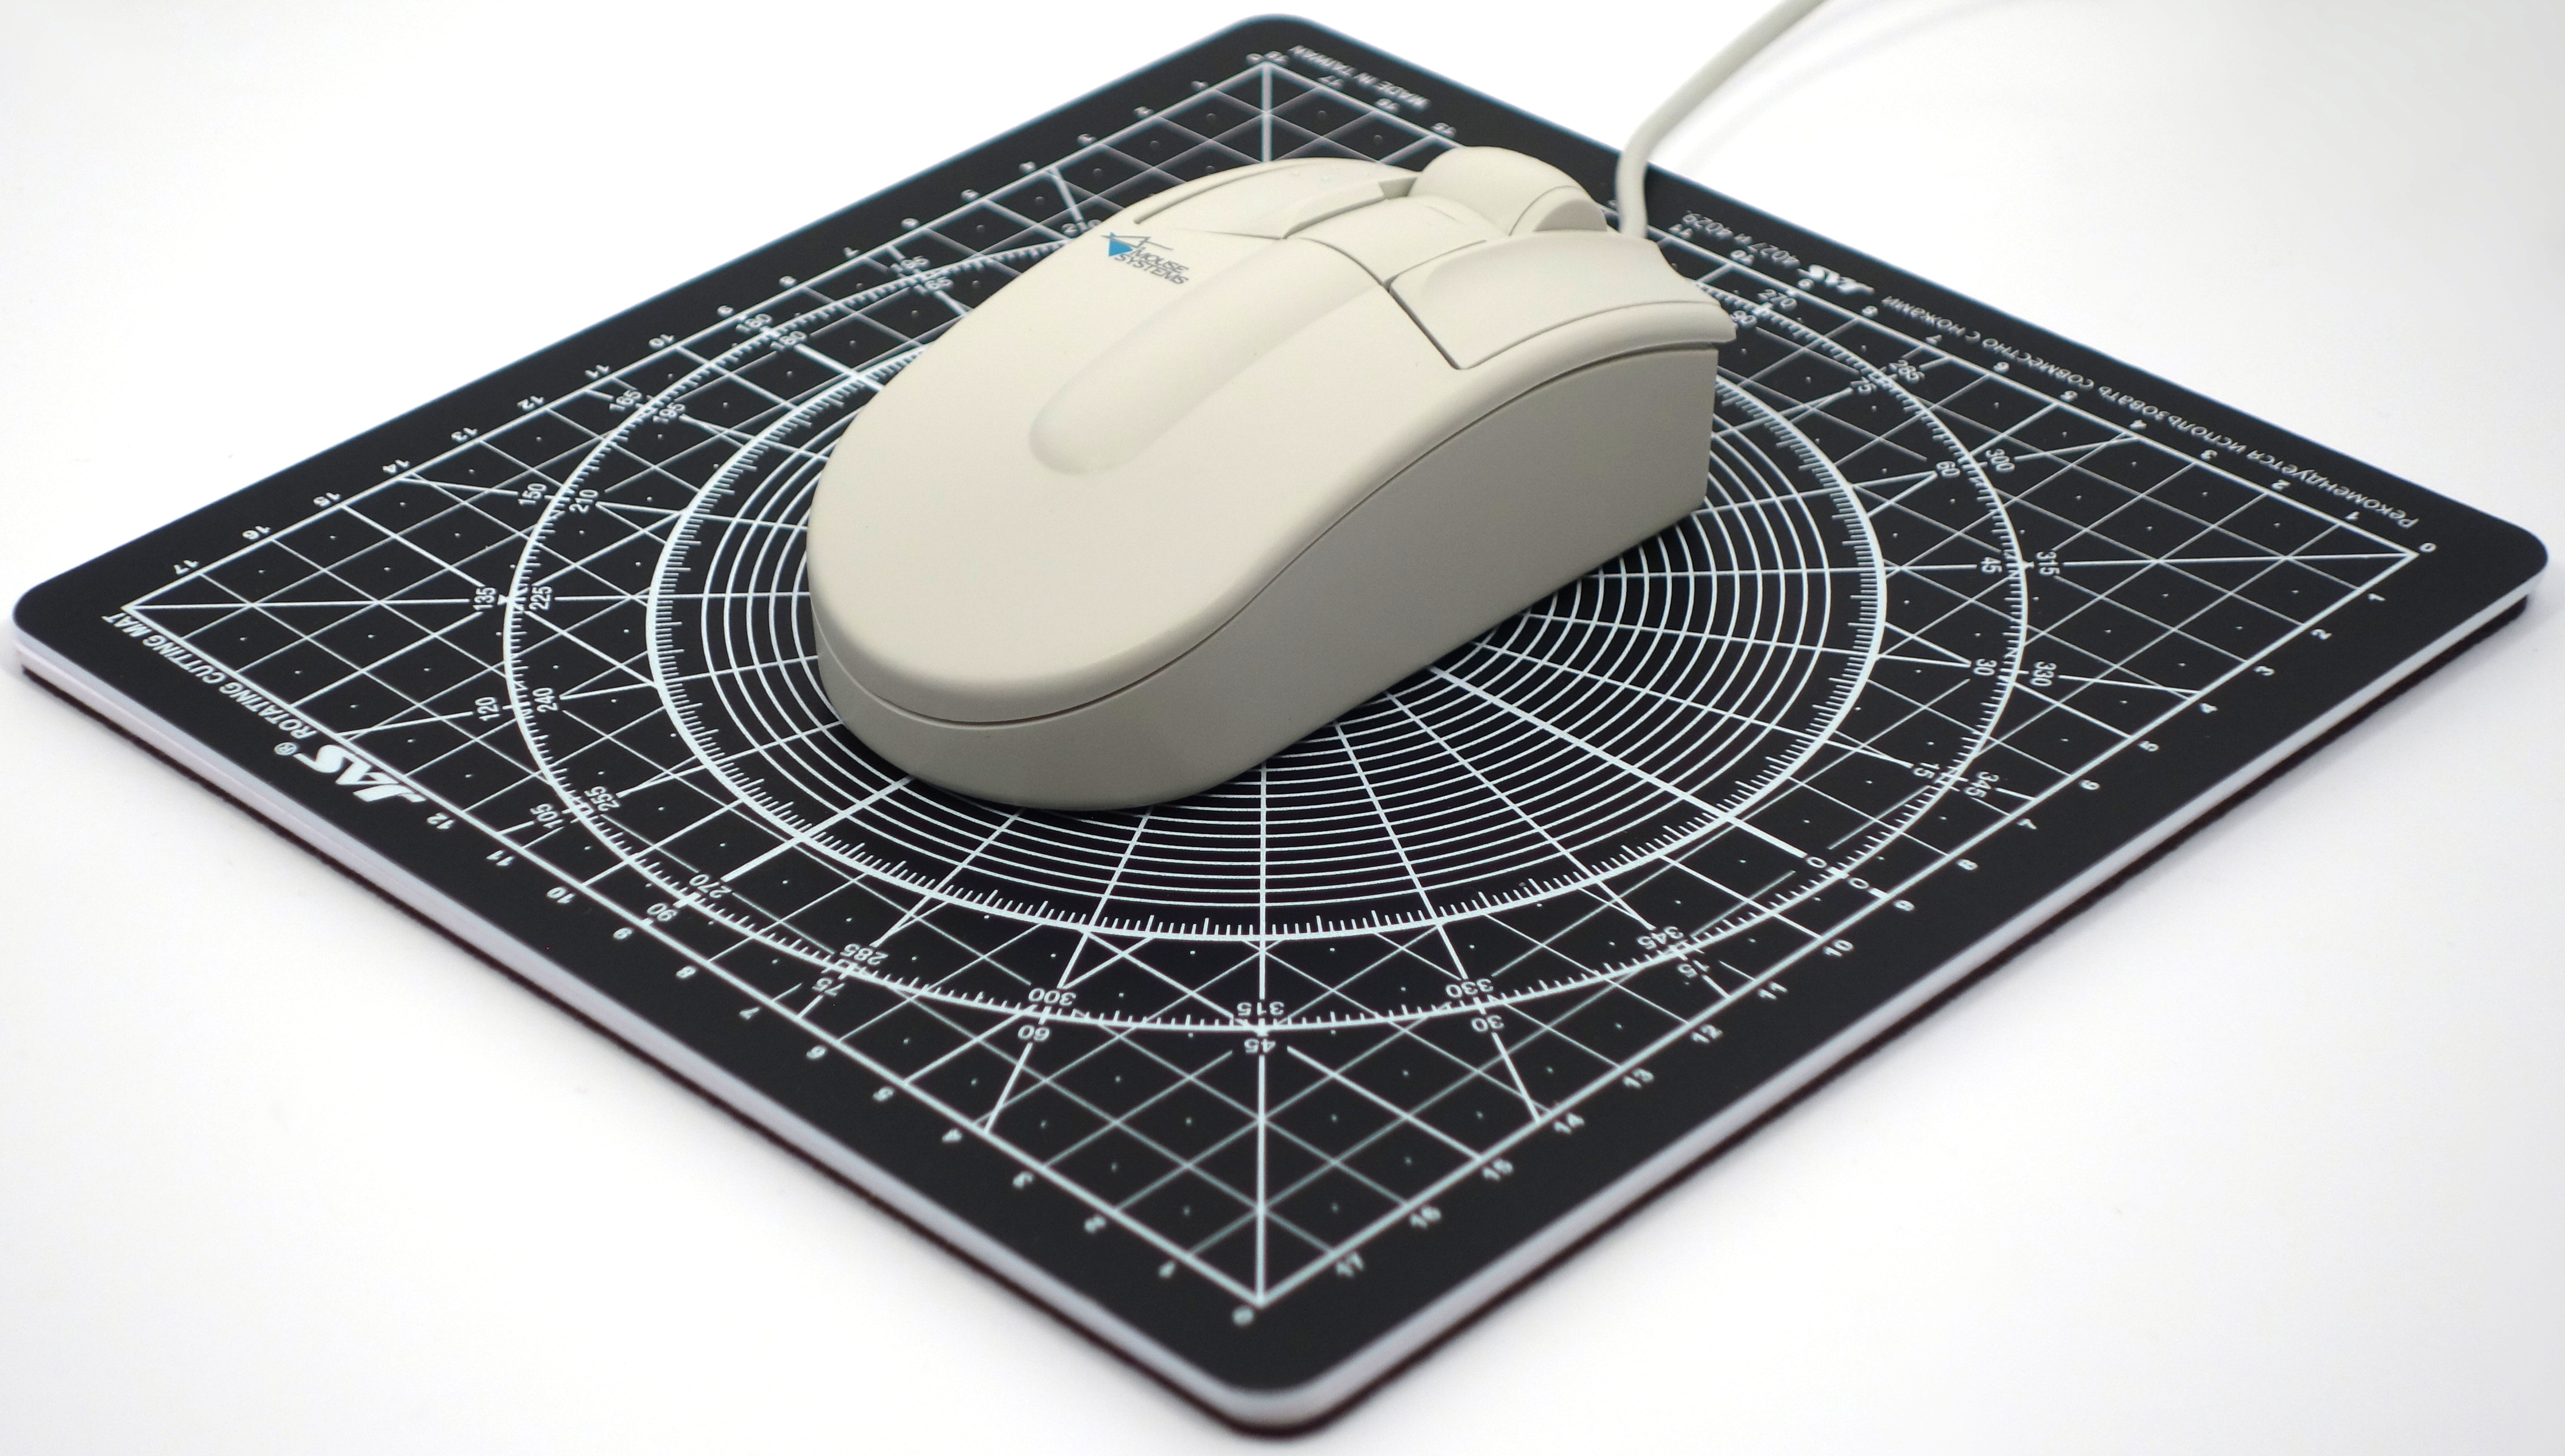
\includegraphics[scale=0.37]{1995_pro_agio_scroll_mouse/size_30.jpg}
    \caption{ProAgio Scroll Mouse on a graduated pad with a grid step of 1~cm}
    \label{fig:ScrollSize}
\end{figure}

Let's quote Eric Michelman from Microsoft, as he describes this in his “The History of the Scroll Wheel” article \cite{ink}:

\textit{Back in 1993, as I was watching many Excel users do their work, I noticed the difficulty they had moving around large spreadsheets. Finding and jumping to different sections was often difficult. I had the idea that perhaps a richer input device would help.
My original idea was the zoom lever. This was simply a lever, presumably for your non-mouse hand (i.e. on the left side of your keyboard if you're right-handed). When you push it away from you the spreadsheet zooms out. When you pull it towards you, it zooms back in.}

\textit{I prototyped this by hooking a joystick up to my computer and using DDE to connect it to Excel for zooming. Using a joystick button along with the stick, I also had it do “data zooming”, which was drilling in and out through Excel outlines.}

\textit{This all seemed useful, so I showed it to the Hardware division at Microsoft. They were initially cool to the idea, which I presented as a zoom lever, and it didn't go anywhere at that point.}

\textit{At this point most people thought it was kind of wacky. Focusing on zooming was a very Excel-centric approach. More specifically, it was a very 2-D centric approach. That is, using an application that presents 2-dimensional data, like a spreadsheet or graphics, it's very useful to zoom in and out. But the other main style of application is a linear flow application like Word, and there it's not as useful. You could do zooming with Word, where zooming out shows you a multi-page view and then you click on a desired page and zoom into it, but that's not as natural as with a spreadsheet or graphics and images.}

\textit{A number of people suggested adding panning and scrolling functionality. In particular I remember Chris Graham saying zooming was just too limiting and it should pan as well. In response to this feedback, I added panning to the prototype, so moving the joystick side-to-side and back-and-forth scrolled Excel in the corresponding direction.}

\textit{Around this time, the hardware guys came back and said that they had considered adding a wheel to the mouse, but they didn't know what it would be used for. Document navigation answered that question, so they said that if I could get Office to support it, they would build it. This really meant Excel and Word since they were the “800 lb gorillas” -- if Excel and Word supported something, then the other Office apps would follow, and if Office as a whole supported something, then everyone else would follow too (this was the early 1993 when Office was the heart of most people's computer usage).}

\begin{figure}[h]
    \centering
    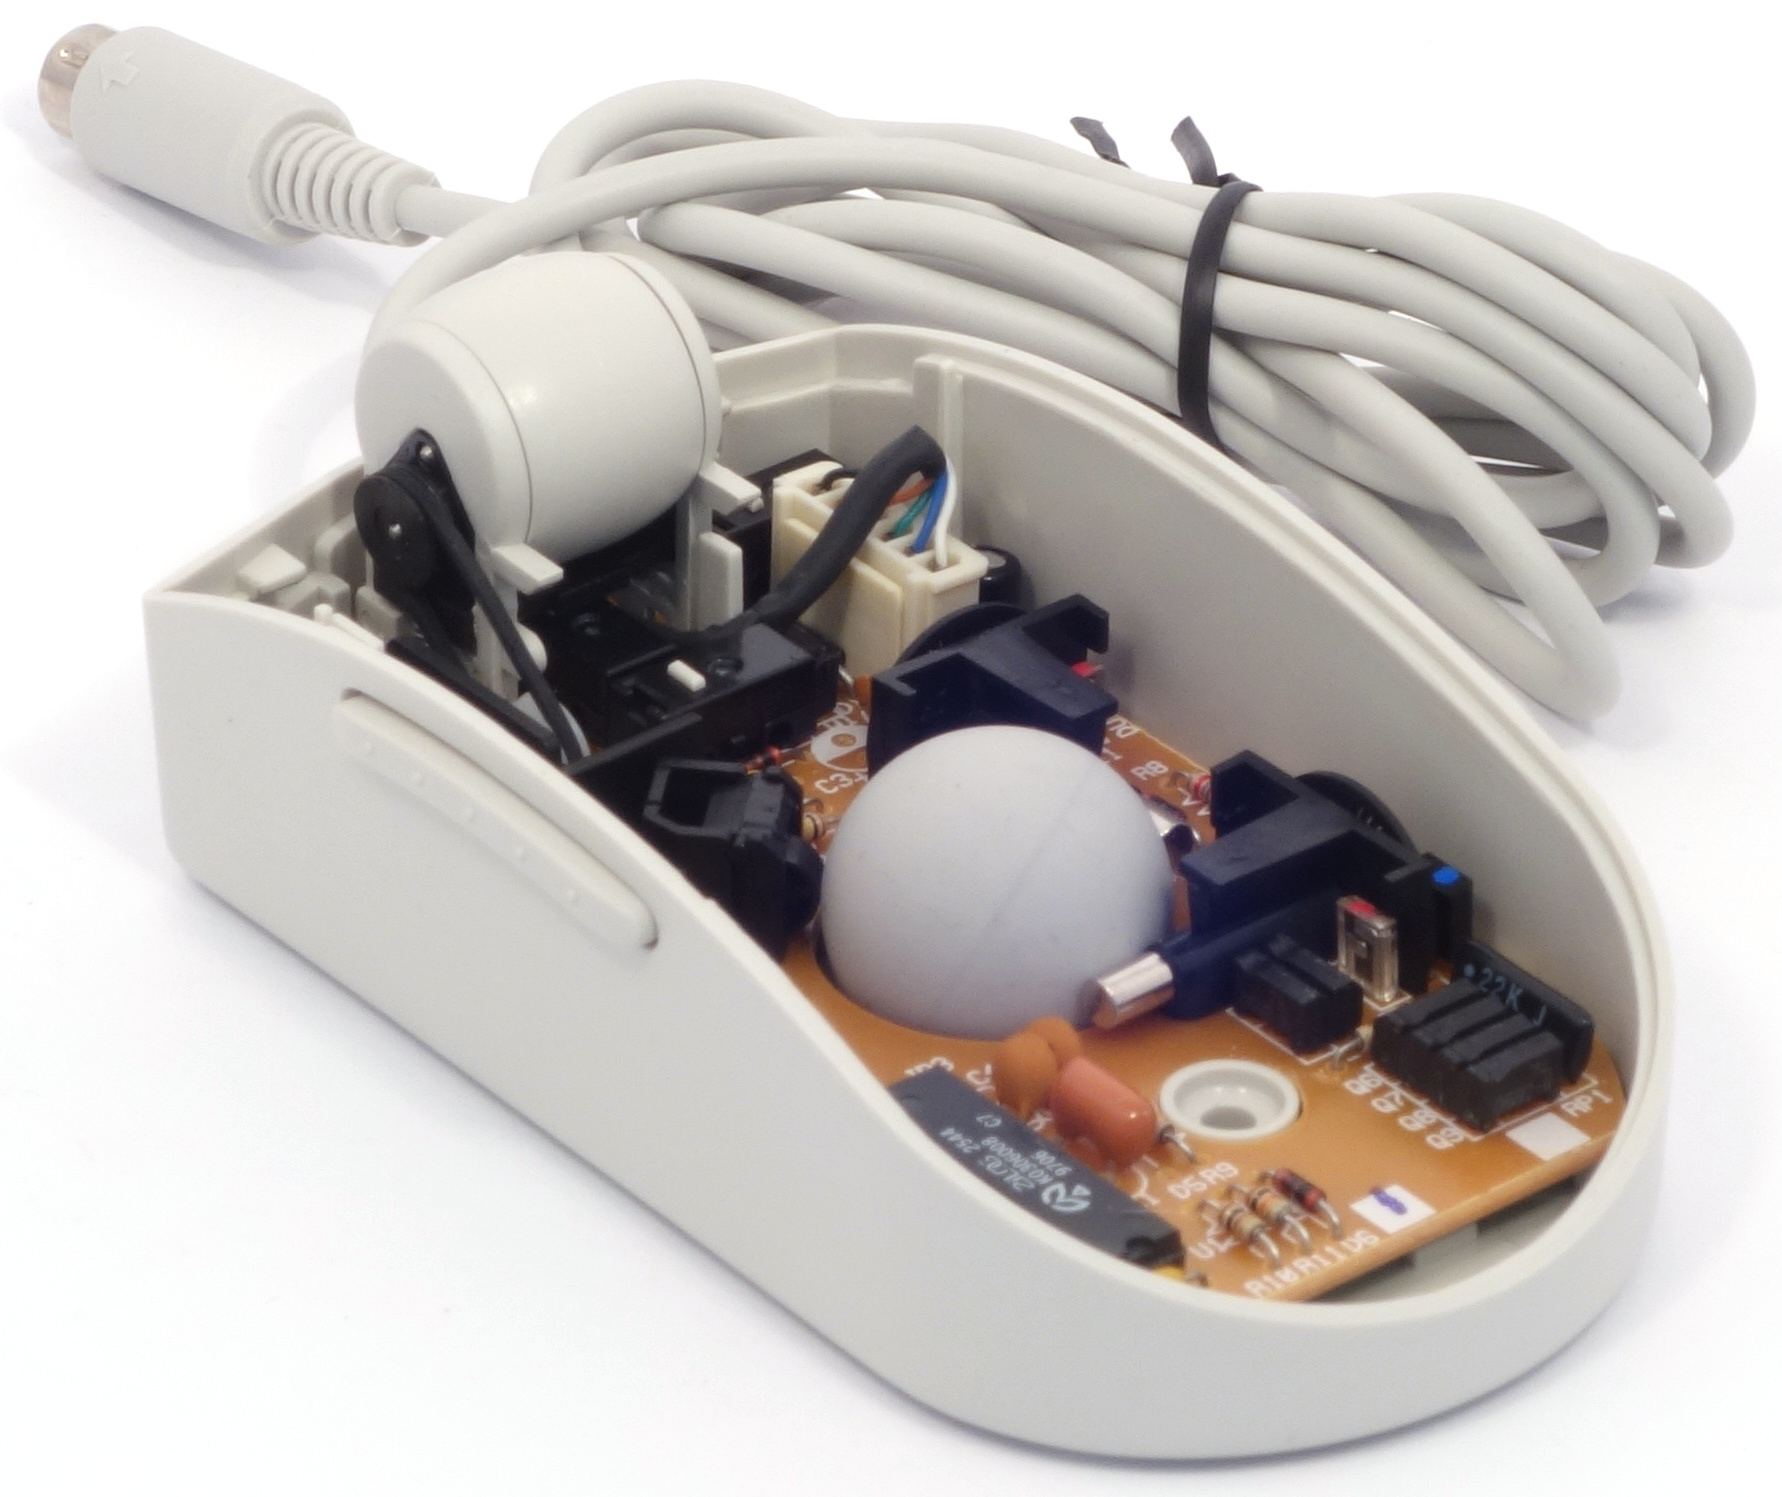
\includegraphics[scale=0.8]{1995_pro_agio_scroll_mouse/inside_30.jpg}
    \caption{ProAgio Scroll Mouse disassembled}
    \label{fig:ScrollInside}
\end{figure}

Mouse internals are shown on figure \ref{fig:ScrollInside}. The mouse uses the traditional opto-mechanical technology (having 400 dots per inch resolution). Also, among the features, it should be noted that the developers used a rubber belt to transmit the wheel rotation, which will be never found in more modern devices.

\begin{thebibliography}{9}
\bibitem {ink} CODING HORROR \url{https://blog.codinghorror.com/meet-the-inventor-of-the-mouse-wheel/}
\bibitem {yt} Mouse Systems ProAgio Scroll Mouse \url{https://www.oldmouse.com/mouse/mousesystems/scroll.shtml}
\end{thebibliography}
\end{document}
